\documentclass[border=5pt]{standalone}
\usepackage{tikz}
\usepackage{amsmath}
\usetikzlibrary{calc}
\begin{document}
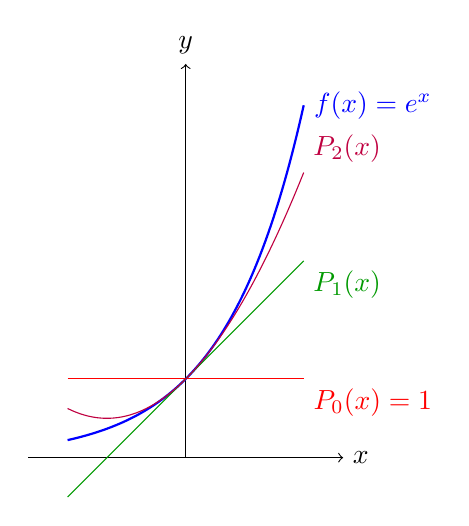
\begin{tikzpicture}[scale=1.0]
\draw[->] (-2,0) -- (2,0) node[right] {$x$};
\draw[->] (0,0) -- (0,5) node[above] {$y$};

% Original function
\draw[thick, domain=-1.5:1.5, samples=100, blue] plot (\x, {exp(\x)}) node[right] {$f(x) = e^x$};

% P_0
\draw[domain=-1.5:1.5, samples=2, red] plot (\x, {1}) node[below right] {$P_0(x) = 1$};

% P_1
\draw[domain=-1.5:1.5, samples=100, green!60!black] plot (\x, {1 + \x}) node[below right] {$P_1(x)$};

% P_2
\draw[domain=-1.5:1.5, samples=100, purple] plot (\x, {1 + \x + \x*\x/2}) node[above right] {$P_2(x)$};

\end{tikzpicture}
\end{document}
